\section{Media over QUIC (MoQ)}\label{sec:moq_bg}

\iffalse % TODO: remove (only notes)

Notes on: https://www.ietf.org/blog/moq-overview/

Target: live streaming, real-time collaboration, gaming, etc.

Good scaling capabilities cause high latency
Low latency systems have poor scaling capabilities

MoQ aims for low latency and high scalability
Built on top of raw QUIC (or WebTransport)

Maybe add quote from https://datatracker.ietf.org/wg/moq/about/

Publisher / Subscriber model
Support for many formats, rate adaptation, cache friendly mechanisms, etc.
Relays function as caches for lower latency and higher quality

Took approaches from RTP (real-time stuff), HLS/DASH (scaling)

If many downstream requests for same data, relay only needs one copy

Media content can be end-to-end encrypted but relay can still access metadata
like priority field - this is similar to our setup.
% TODO: how can these fields still be accessed? are they just not encrypted?
Priority can be used when caching or when forwarding under congestion.
The MoQ can drop or delay certain media if necessary.

VoD consumption >> live streaming but live makes up most of peak traffic

MoQ will have great influence on real-time collaboration infrastructure like 
Zoom, Teams, etc.~and live streaming platforms like Twitch, YouTube, etc. 

low latency, high fan out, high scalability is pretty much ideal for most apps.

(Also psychological improvement since latency problems tend to be blamed on the 
other party, not the network.) % TODO: prolly no fit in this section?
https://blog.webex.com/hybrid-work/how-latency-harms-collaboration/

\fi

% \subsection{What is Media over QUIC (MoQ)?} % TODO: maybe not needed
On the application layer, we will use the Media over QUIC (MoQ) protocol which 
is, as of summer 2024, still in the process of standardization by the IETF~\parencite{moq-charter}.
MoQ targets live-streaming applications like Twitch or YouTube-Live and real-time collaboration 
applications like Zoom, Microsoft Teams, or Google Meet.
It is built on top of the QUIC protocol with the possibility of using WebTransport
for browser support.
A general publisher/subscriber model is used, and the draft tries to combine
performant approaches from protocols like RTP (for real-time features) and HLS/DASH
(for scalability).

\subsection{Solving Scaling versus Latency}
For a long time now, there have been two different camps with regard to media-data-
transmission-protocols and -setups.
One is heavily focused on low latency, while the other aims for high scalability~\parencite{what-is-moq}.
Systems of the former kind include real-time collaboration tools like aforementioned Zoom, Teams, or Meet.
The latter ones are often huge platforms like Twitch, YouTube, or Netflix, which need to 
reach millions of users at the same time.
The one thing both have in common is that it turns out to be difficult to incorporate both 
low latency and high scalability into the system at the same time~\parencite{what-is-moq}.
The MoQ protocol tries to solve this by providing a setup that is both low-latency and
highly scalable.
To achieve this, it supports performance-enhancing approaches like relay caching or support 
for adaptive rate mechanisms. % TODO: other things that are used to achieve this?

\subsection{Design of a MoQ Relay}
The charter for the IETF working group~\parencite{moq-charter} describes what MoQ, and therefore also a relay 
that wants to meet the MoQ requirements, needs to support.
These requirements for the publication- and distribution-setup mention the support of 
multiple formats, dynamic rate adaption mechanisms (e.g.~used for congestion handling)
as well as cache-friendly mechanisms.

\begin{figure}[H]
    \centering
    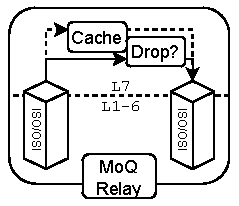
\includegraphics[width=0.3\textwidth]{figures/02_background/moq-relay.drawio.pdf}
    \caption[MoQ relay architecture]{MoQ relay architecture.}\label{fig:moq-relay-architecture}
\end{figure}

Figure~\ref{fig:moq-relay-architecture} gives a visualization of the rough architecture
of a MoQ relay.
It hints at key components like the relay level cache and the congestion handling
mechanism.
What one can also infer is the place of MoQ in the OSI-model namely at the application
layer, which itself builds on top of lower-level protocols like QUIC, UDP, IP, and Ethernet.
In figure~\ref{fig:relay-caching} one can see a comparison between a traditional non-caching
relay and a caching MoQ-relay.
The latter lowers the traffic between server and relay in case the same data is requested
by multiple clients.

\vspace{0.5cm}
\begin{figure}[H]
    \centering
    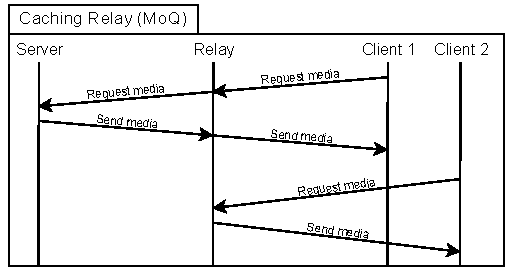
\includegraphics[width=1\linewidth]{figures/02_background/relay-caching.drawio.pdf}
    \caption[Cache related relay traffic]{Multiple clients requesting data for caching and non-caching relay.}\label{fig:relay-caching}
\end{figure}

This caching mechanism fits quite naturally into our proposed eBPF setup since we will need to 
communicate packet data between kernel- and user-space anyway to keep the QUIC library in a 
consistent state.
In addition to that, the congestion-handling functionality of the MoQ relay can also
be integrated fairly easily within eBPF\@.
This is because packet dropping is ultimately one of the main use cases of plain eBPF 
programs and, as such, easy to implement.
In a later section we will go into detail on how the eBPF setup actually uses mechanisms like 
priority fields for this and how those meet the standard specifications.

\subsection{moqtransport}
To use the MoQ protocol in our setup, we will make use of a library that implements 
the MoQ transport protocol (moqtransport or MoQT) in Go~\parencite{priority-moqtransport-repo}
The goal of MoQT is to define a media transport protocol that is operating on top
of QUIC and WebTransport, which is providing the concrete designs that the charter of 
the MoQ working group is aiming for.
This includes, for example, the actual structure of the different message types or error handling in case 
of a wrong state.
As of writing this thesis, the MoQT draft is in its fifth version~\parencite{draft-moqtransport}.

% Besides that, the fast-relay implementation will also make use of the moqtransport library.
% This library brings the ``Media over QUIC'' (MoQ) protocol to Go and will be used as a media transport protocol 
% when looking at the impact of fast-relays on adaptive real-time video streaming.
% The MoQ protocol is being standardized by the IETF since July 2023 and has yet to be finalized. 